\begin{figure}[H]
\centering
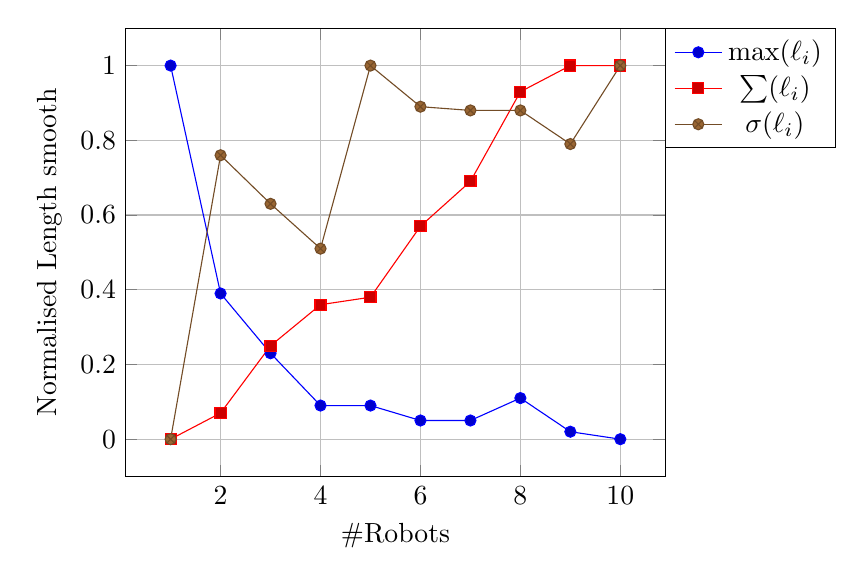
\begin{tikzpicture}
	\begin{axis}[
%		height=9cm,
%		width=9cm,
		grid=major,
                legend style = {at={(1,1)}, anchor=north west},
		xlabel=\#Robots,
		ylabel=Normalised Length
		smooth,
		tension=0.3
	]

	\addplot coordinates {
(1, 1.00)
(2, 0.39)
(3, 0.23)
(4, 0.09)
(5, 0.09)
(6, 0.05)
(7, 0.05)
(8, 0.11)
(9, 0.02)
(10, 0.00)
	};
	\addlegendentry{$\max(\ell_i)$}

	\addplot coordinates {
(1, 0.00)
(2, 0.07)
(3, 0.25)
(4, 0.36)
(5, 0.38)
(6, 0.57)
(7, 0.69)
(8, 0.93)
(9, 1.00)
(10, 1.00)
	};
	\addlegendentry{$\sum(\ell_i)$}

	\addplot coordinates {
(1, 0.00)
(2, 0.76)
(3, 0.63)
(4, 0.51)
(5, 1.00)
(6, 0.89)
(7, 0.88)
(8, 0.88)
(9, 0.79)
(10, 1.00)
	};
	\addlegendentry{$\sigma(\ell_i)$}
	\end{axis}
\end{tikzpicture}
\caption[Perform. indexes increasing the \#robots, city map using VRP]{\mbox{Performance indexes increasing the num. of robots, city map using VRP}}
\end{figure}